% !TEX root = pocs-2-project-revtex4.tex

%% replace 'papertag' with short distinct tag
%% - helps with distinction for inclusion in other documents
%% - always

%% procedure for figures:
%% adding directory figures/localized/
%% before figures in includegraphics
%% commands forces search and localize

\usepackage{booktabs}

\section{Introduction}
\label{sec:papertag.introduction}

\begin{figure}[tp!]
  \centering
    
\includegraphics[width=0.5\columnwidth]{figures/localized/Garak.jpg}
  \caption{
    Garak, tailor and retired (?) spymaster.
  }
  \label{fig:papertag.}
\end{figure}

\section{Description of data sets}
\label{sec:papertag.data}

Transcripts of all episodes of \textit{Star Trek: The Original Series} (TOS), \textit{The Next Generation} (TNG) and \textit{Deep Space Nine} (DS9), as obtained from \href{http://chakoteya.net/StarTrek/index.html}{chakoteya.net} in February 2023. These are the first three live-action series of the Star Trek franchise. Further information about the corpus can be found in table \ref{table:series-comparison}.

\begin{table}
\centering
\begin{tabular}{l|c|c|c}
Series & Original Run & \# Episodes & Words per Episode \\
\hline
TOS & 1966--1969 & 79 & [Value] \\
TNG & 1987--1994 & 178 & [Value] \\
DS9 & 1993--1999 & 176 & [Value] \\
\end{tabular}
\caption{Comparison of Star Trek Series: TOS, TNG, and DS9}
\label{table:series-comparison}
\end{table}

\begin{figure}
  \centering
  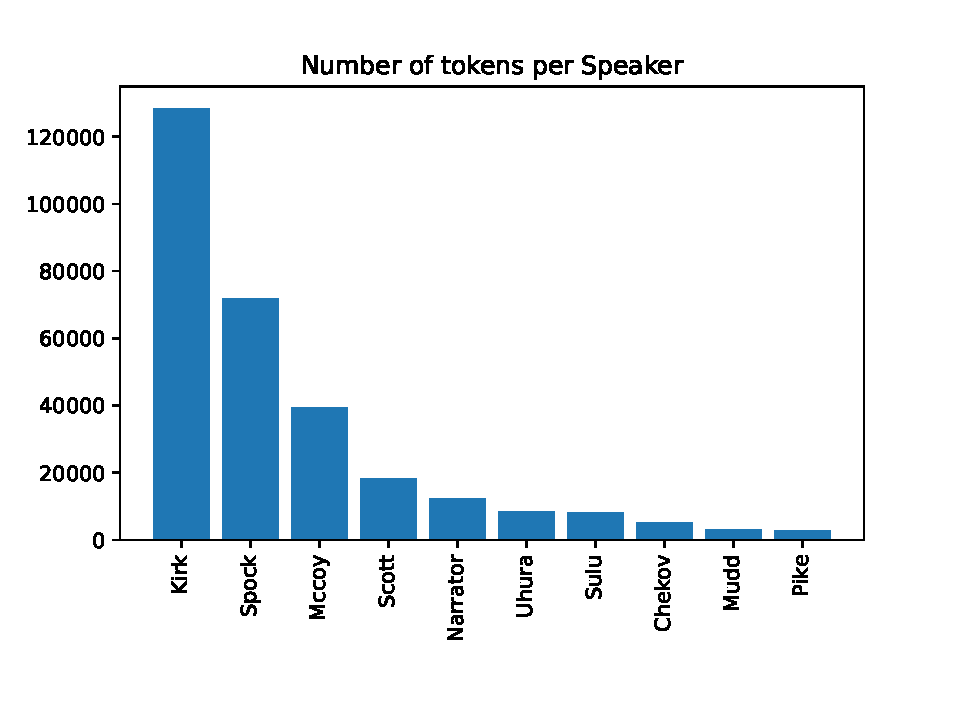
\includegraphics[width=\columnwidth]{figures/localized/tos_group_sizes.pdf}
  \caption{Number of words per speaker for the 10 most prolific speakers in \textit{Star Trek: The Original Series}.}
  \label{fig:tos_group_sizes}
\end{figure}

\begin{figure}
  \centering
  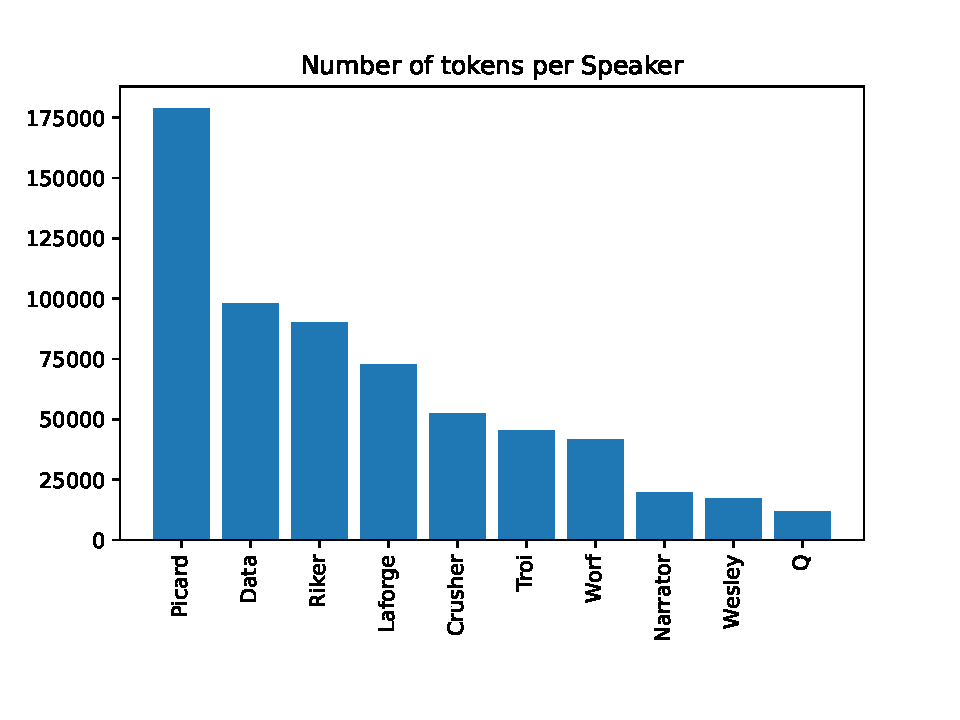
\includegraphics[width=\columnwidth]{figures/localized/tng_group_sizes.pdf}
  \caption{Number of words per speaker for the 10 most prolific speakers in \textit{Star Trek: The Next Generation}.}
  \label{fig:tng_group_sizes}
\end{figure}

\begin{figure}
  \centering
  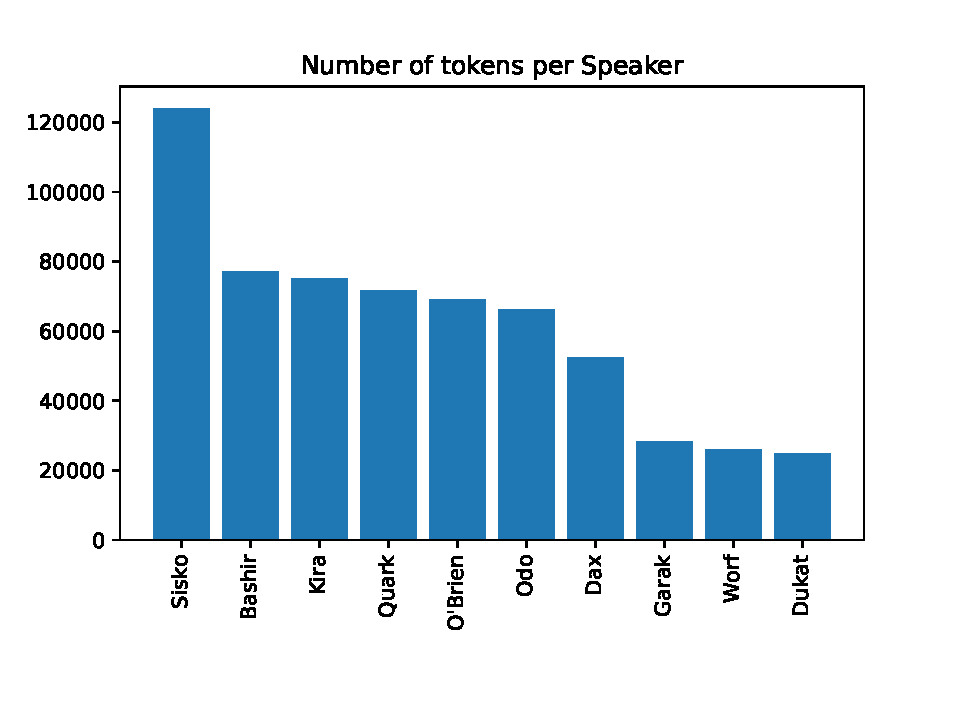
\includegraphics[width=\columnwidth]{figures/localized/ds9_group_sizes.pdf}
  \caption{Number of words per speaker for the 10 most prolific speakers in \textit{Star Trek: Deep Space Nine}.}
  \label{fig:ds9_group_sizes}
\end{figure}

Clearly visible in \ref{fig:tos_group_sizes}, \ref{fig:tng_group_sizes} and \ref{fig:ds9_group_sizes}: The respective Captain sticks out as the main character. But while TOS follows what looks like a power-law distribution, TNG has a stronger notion of a core cast, and DS9 even more so.

\begin{figure}
  \centering
  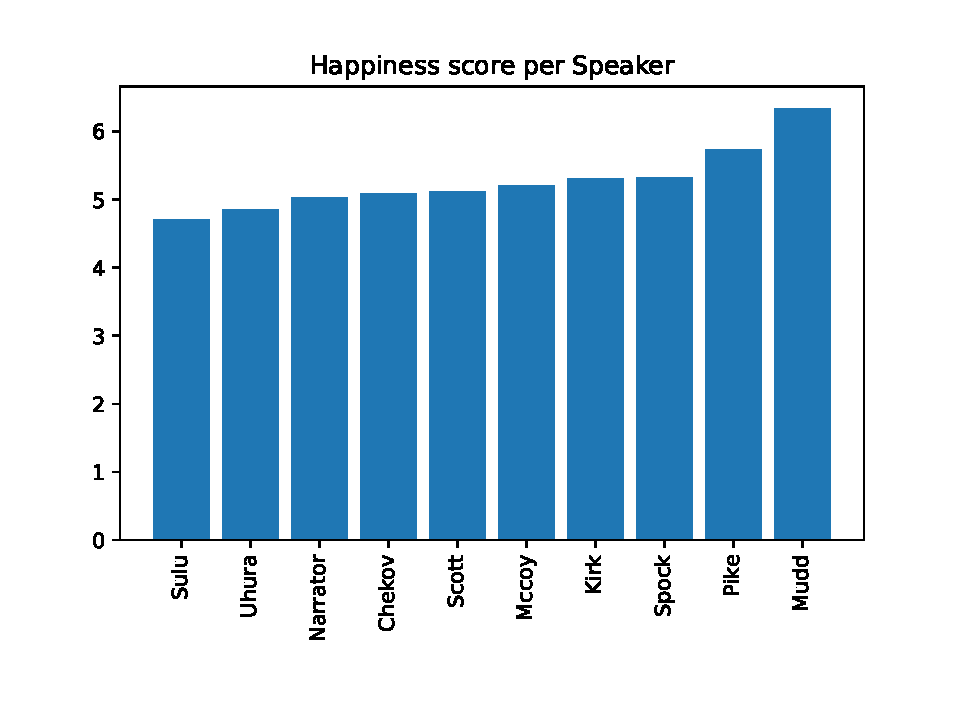
\includegraphics[width=\columnwidth]{figures/localized/tos_happiness_scores.pdf}
  \caption{Happiness score comparison of the 10 most prolific speakers in \textit{Star Trek: The Original Series}.}
  \label{fig:tos_happiness}
\end{figure}

\begin{figure}
  \centering
  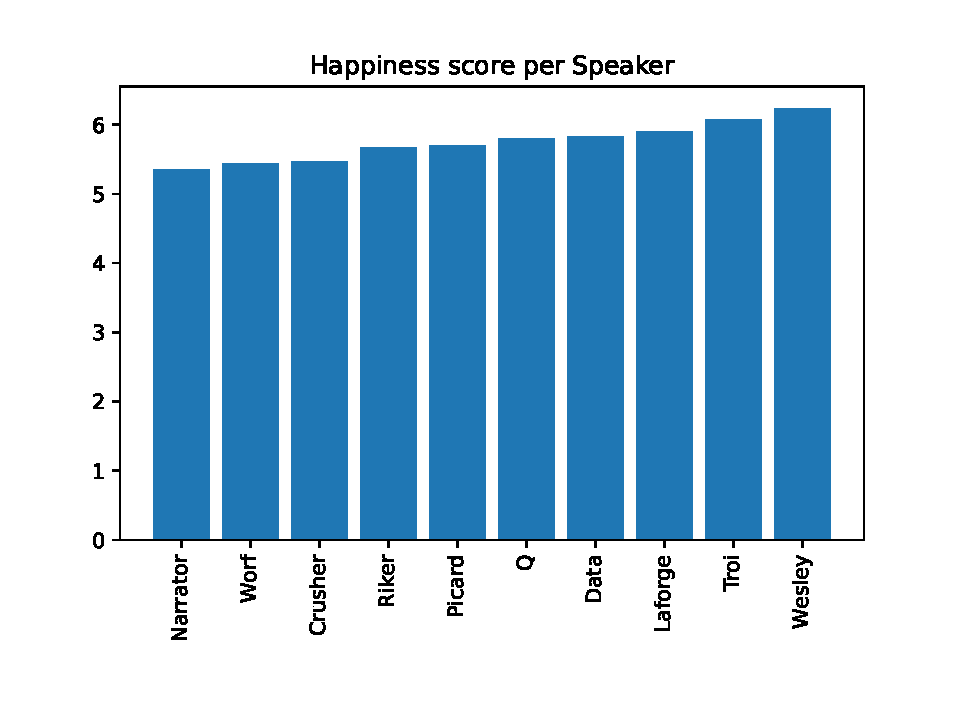
\includegraphics[width=\columnwidth]{figures/localized/tng_happiness_scores.pdf}
  \caption{Happiness score comparison of the 10 most prolific speakers in \textit{Star Trek: The Next Generation}.}
  \label{fig:tng_happiness}
\end{figure}

\begin{figure}
  \centering
  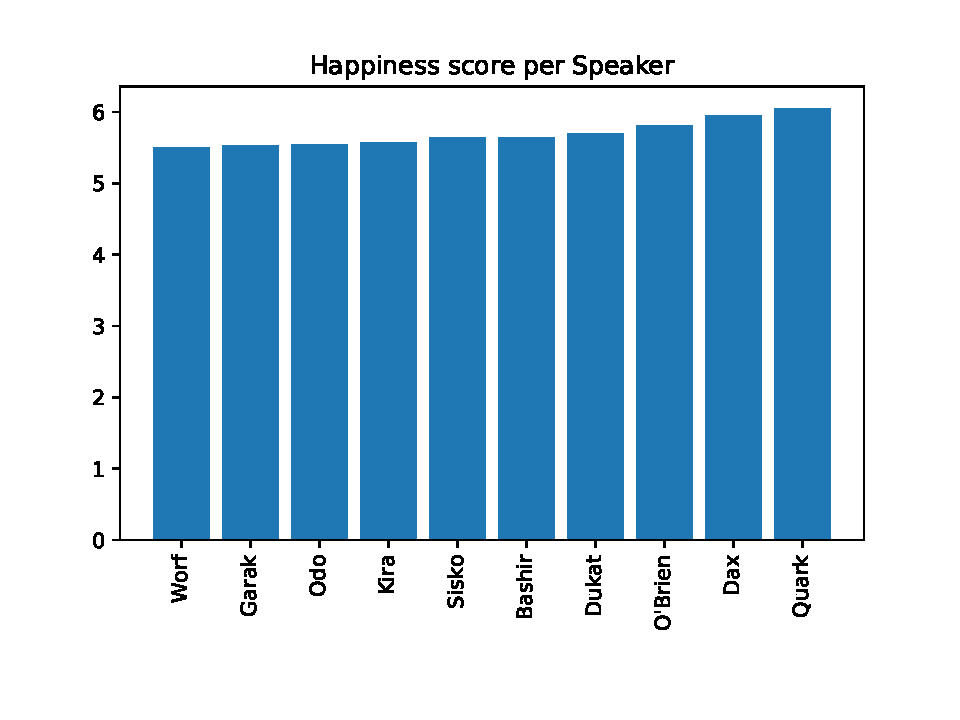
\includegraphics[width=\columnwidth]{figures/localized/ds9_happiness_scores.pdf}
  \caption{Happiness score comparison of the 10 most prolific speakers in \textit{Star Trek: Deep Space Nine}.}
  \label{fig:ds9_happiness}
\end{figure}

\section{Model}
\label{sec:papertag.model}

\section{Results}
\label{sec:papertag.results}

\todo{Explain what we found}

\begin{figure}
    \centering
    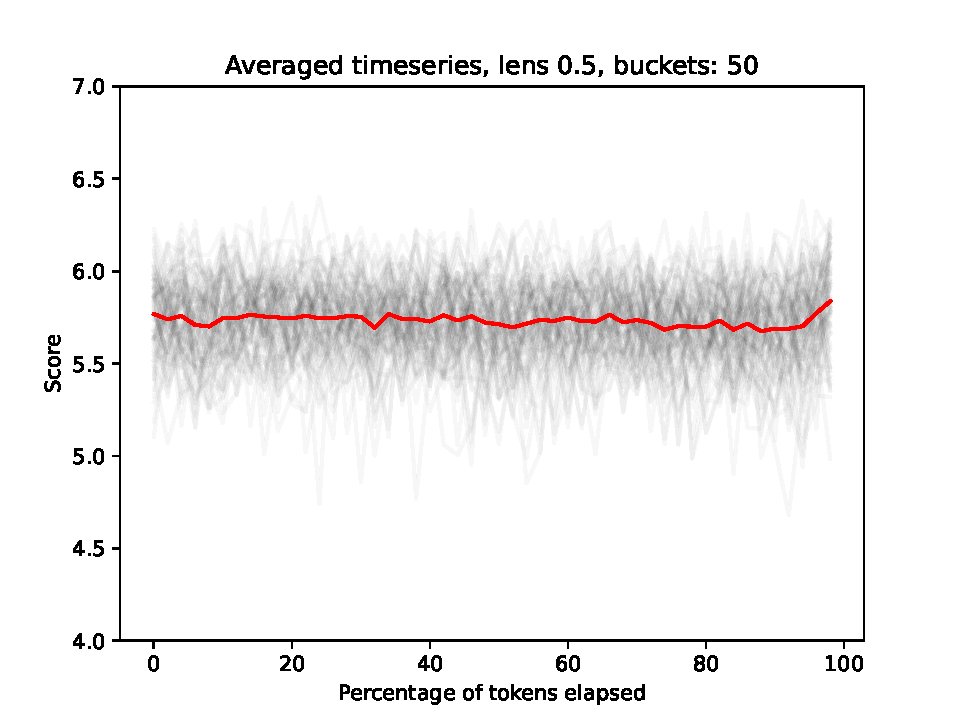
\includegraphics[width=\columnwidth]{figures/localized/average_episode_tos.pdf}
    \caption{Happiness timeseries of the average episode of Star Trek: The Original Series. Episodes are scaled to the length of the shortest episode. All episodes plotted in black, the red line is the average.}
    \label{fig:average_episode_tos}
\end{figure}

\begin{figure}
    \centering
    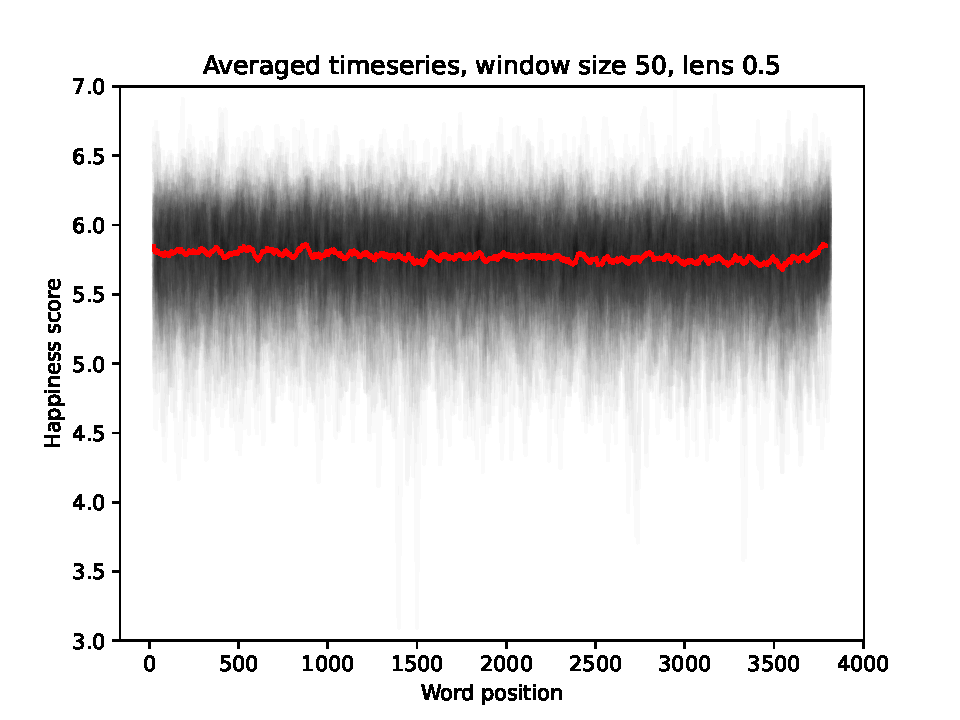
\includegraphics[width=\columnwidth]{figures/localized/average_episode_tng.pdf}
    \caption{Happiness timeseries of the average episode of Star Trek: The Next Generation. Episodes are scaled to the length of the shortest episode. All episodes plotted in black, the red line is the average.}
    \label{fig:average_episode_tng}
\end{figure}

\begin{figure}
    \centering
    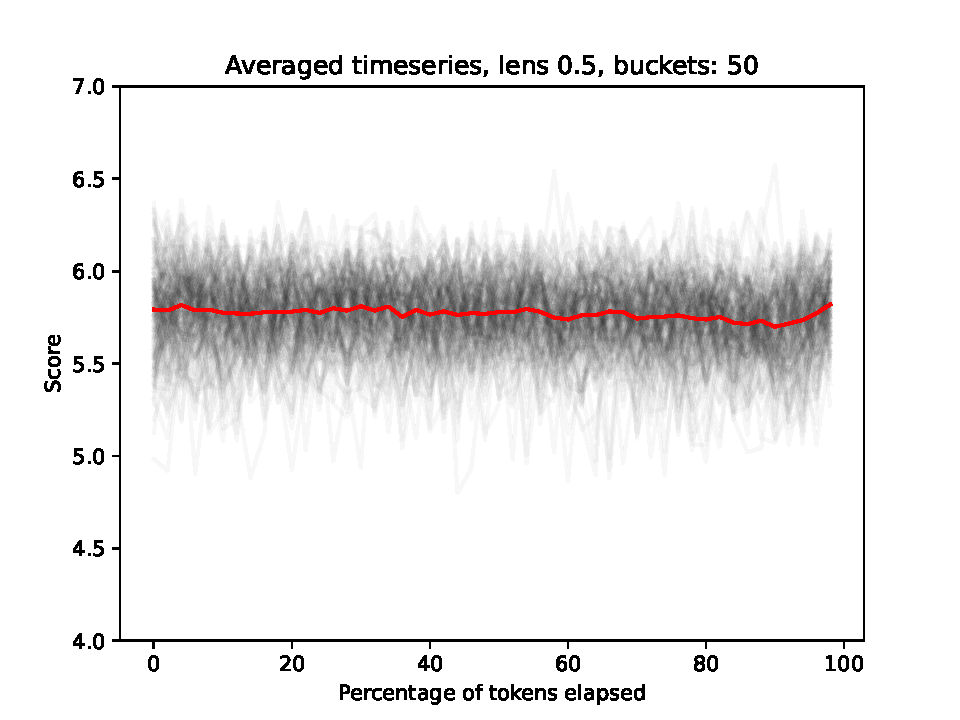
\includegraphics[width=\columnwidth]{figures/localized/average_episode_ds9.pdf}
    \caption{Happiness timeseries of the average episode of Star Trek: Deep Space Nine. Episodes are scaled to the length of the shortest episode. All episodes plotted in black, the red line is the average.}
    \label{fig:average_episode_ds9}
\end{figure}

Visible in \ref{fig:average_episode_tos}, \ref{fig:average_episode_tng} and \ref{fig:average_episode_ds9}: The episodes usually have a happy end in all three series. Average happiness is comparable overall.

\section{Concluding remarks}
\label{sec:papertag.concludingremarks}

\todo{Bring it home.}

\section{Methods}
\label{sec:papertag.methods}

\todo{Add methods.}
